\documentclass[11pt,mathserif]{beamer}
\usepackage{graphicx,amsmath,amssymb,psfrag,minted}
\usepackage{tikz}
\usetikzlibrary{positioning,calc,shapes,arrows}
% Define block styles XXX
\tikzstyle{block} = [rectangle, draw,
    text width=8em, text centered, minimum height=5em]
\tikzstyle{line} = [draw, -latex',line width=1mm]

% \input defs.tex

%% formatting

\mode<presentation>
{
\usetheme{default}
}
\setbeamertemplate{navigation symbols}{}
\usecolortheme[rgb={0.13,0.28,0.59}]{structure}
\setbeamertemplate{itemize subitem}{--}
\setbeamertemplate{frametitle} {
	\begin{center}
	  {\large\bf \insertframetitle}
	\end{center}
}

\newcommand\footlineon{
  \setbeamertemplate{footline} {
    \begin{beamercolorbox}[ht=2.5ex,dp=1.125ex,leftskip=.8cm,rightskip=.6cm]{structure}
      \footnotesize \insertsection
      \hfill
      {\insertframenumber}
    \end{beamercolorbox}
    \vskip 0.45cm
  }
}
\footlineon

%% begin presentation

\title{\large \bfseries Linear Least Squares Modeling in Haskell}

\author{Tri Dao\\[3ex]
CS 240H\\
Stanford University}

\date{March 16, 2016}

\begin{document}

\frame{
\thispagestyle{empty}
\titlepage
}

\begin{frame}{Least squares problem}

\begin{itemize}
  \item The \emph{least squares problem} is
  \[
    \begin{array}{ll}
      \mbox{minimize} & \|Ax-b\|^2
    \end{array}
  \]
  \item Solution of least squares problem is
  \[
    \hat x = (A^T A)^{-1} A^T b = A^\dagger b
  \]
\end{itemize}
\end{frame}

\begin{frame}{Example}
\begin{center}
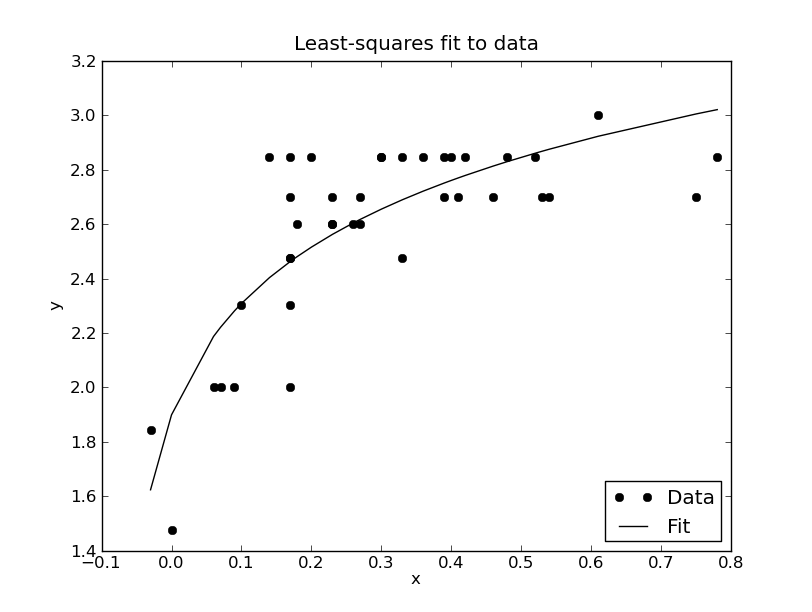
\includegraphics[width=\linewidth]{figures/data_fit.png}
\end{center}
\end{frame}

\begin{frame}{Constrained least squares problem}
\begin{itemize}
  \item The (linearly) \emph{constrained least squares problem} is
  \[
    \begin{array}{ll}
      \mbox{minimize} & \|Ax-b\|^2 \\
      \mbox{subject to} & Cx = d
    \end{array}
  \]
  \item Solution of the constrained least squares problem is
  \[
    \left[\begin{array}{c} \hat x \\ z \end{array}\right] =
    \left[\begin{array}{cc} 2A^TA & C^T \\ C & 0 \end{array}\right]^{-1}
    \left[\begin{array}{c} 2A^Tb \\ d \end{array}\right]
  \]
\end{itemize}
\end{frame}

\begin{frame}{Least squares modeling}
\only<1>{\inputminted{haskell}{app/example1.hs}}
\only<2>{\inputminted{haskell}{app/example2.hs}}
\end{frame}

\begin{frame}{Modeling language}
\vfill
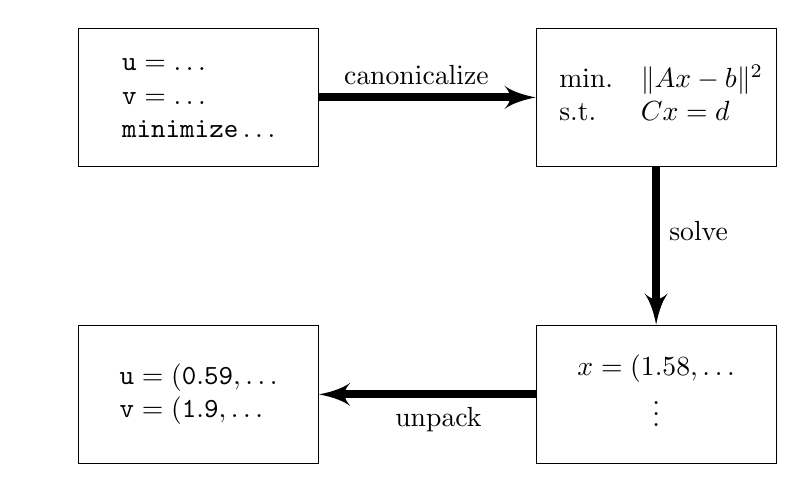
\begin{tikzpicture}[auto]
    % Place nodes
    \node (left_up) {};
    % \node [below=1cm of left_up] (left_down) {};
    \node [block,right=4mm of left_up] (code) {$\begin{array}{l}
    \tt{u = \ldots} \\
    \tt{v = \ldots} \\
    \tt{minimize \ldots}
    \end{array}$};
    \node [block, right =2.75cm of code] (cone) {$\begin{array}{ll}
\mbox{min.}  &\|Ax-b\|^2 \\
\mbox{s.t.} &Cx = d
\end{array}$};
    \node [block, below =2cm of cone] (sltn) {$\begin{array}{c}
x = (1.58,\ldots \\
 \vdots
\end{array}$};
    \node [block, left =2.75cm of sltn] (unpack) {$\begin{array}{l}
    \tt{u = (0.59,\ldots}\\
    \tt{v = (1.9,\ldots}
    \end{array}$};
\path [line] (code) -- node {canonicalize} ++(4,0) -- (cone);
\path [line] (cone) -- node {solve} ++(0,-2.5) -- (sltn);
\path [line] (sltn) -- node {unpack} ++(-4,0) -- (unpack);
\end{tikzpicture}
\vfill
\end{frame}

\begin{frame}{Image de-blurring}
\begin{itemize}
\item $x$ is an image, $A$ is a blurring operator, and $y=Ax+v$
is a blurred, noisy image
\item least-squares de-blurring: choose $x$ to minimize
\[
 \|Ax -  y\|^2 + \lambda (\|D_\mathrm v x\|^2 + \|D_\mathrm h x\|^2)
\]
$D_\mathrm v$, $D_\mathrm h$ are vertical and horizontal
differencing operations
\inputminted{haskell}{app/example3.hs}
\item $\lambda$ controls smoothing of de-blurred image
\end{itemize}

\end{frame}

\begin{frame}{Example}
\begin{itemize}
\item left: blurred, noisy image
\item right: regularized inversion with
$\lambda = 0.007$
\end{itemize}

\hspace*{\fill}
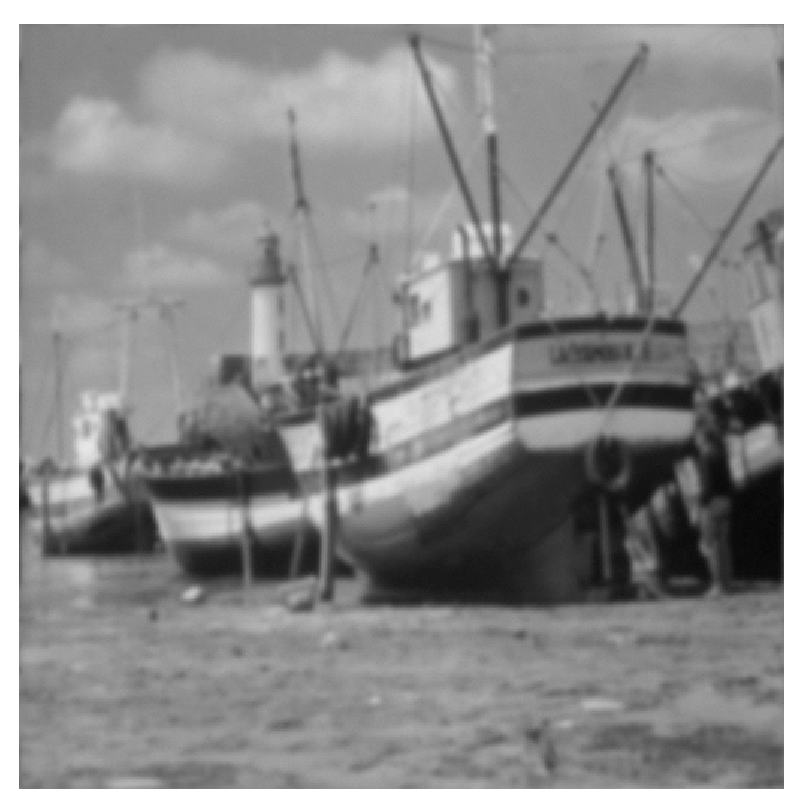
\includegraphics[width=.4\linewidth]{figures/boat_blurred.eps}
\hspace*{\fill}
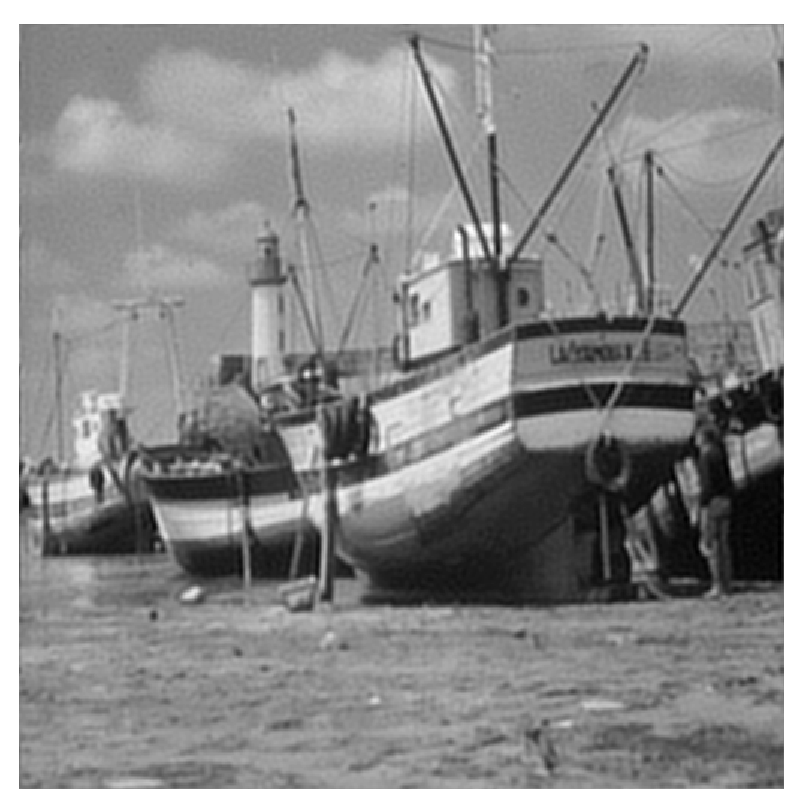
\includegraphics[width=.4\linewidth]{figures/boat_deblurred.eps}
\hspace*{\fill}
\end{frame}

\end{document}
